\chapter{Implementation}
\label{chap:implementation}

This chapter describes the implementation of the Gateway Dashboard system, organised into two main sections. Section~\ref{sec:backend} covers the backend services: Section~\ref{sec:authentication_and_sso} details the authentication system with Single Sign-On support, and Section~\ref{sec:payment} describes the payment and subscription management infrastructure. Section~\ref{sec:frontend} covers the frontend dashboard integration: Section~\ref{sec:frontend_overview} presents the frontend architecture, Section~\ref{sec:frontend_auth} explains the authentication user experience, Section~\ref{sec:frontend_routing} describes routing and navigation guards, and Section~\ref{sec:frontend_subscription} details the subscription management interface.

% ============================================================
% PART 1: BACKEND IMPLEMENTATION
% ============================================================
\section{Backend Implementation}
\label{sec:backend}

The backend is built with NestJS, a modular Node.js framework that provides a well structured foundation for building scalable server side applications. The backend is organised into distinct modules, each responsible for a specific domain of functionality. Section~\ref{sec:authentication_and_sso} describes the authentication system with SSO support, and Section~\ref{sec:payment} covers the payment and subscription management system.

\input{tex/ch4_implementation/01_sso}
\input{tex/ch4_implementation/02_payment}

% ============================================================
% PART 2: FRONTEND IMPLEMENTATION
% ============================================================
\section{Frontend Dashboard Integration}
\label{sec:frontend}

The Gateway Dashboard is an existing Single Page Application (SPA) built with Vue.js 3 and Vuetify. This project extends the dashboard by integrating several new pages that support SSO authentication, subscription management, and administrative controls. Section~\ref{sec:frontend_overview} presents the overall frontend architecture, Section~\ref{sec:frontend_auth} describes the authentication user experience, Section~\ref{sec:frontend_routing} covers the routing and navigation guard system, and Section~\ref{sec:frontend_subscription} details the subscription management interface.

\subsection{Overview}
\label{sec:frontend_overview}

The Gateway Dashboard is a modern web application built with Vue.js 3, providing an intuitive management interface for the Speech Gateway API. The application supports user authentication, subscription management, and administrative controls through a responsive single page application architecture.

\subsubsection{Frontend Architecture}

Figure~\ref{fig:frontend_architecture_simple} illustrates the layered architecture of the frontend application, showing the four main layers and how data flows between them.

\begin{figure}[H]
\centering
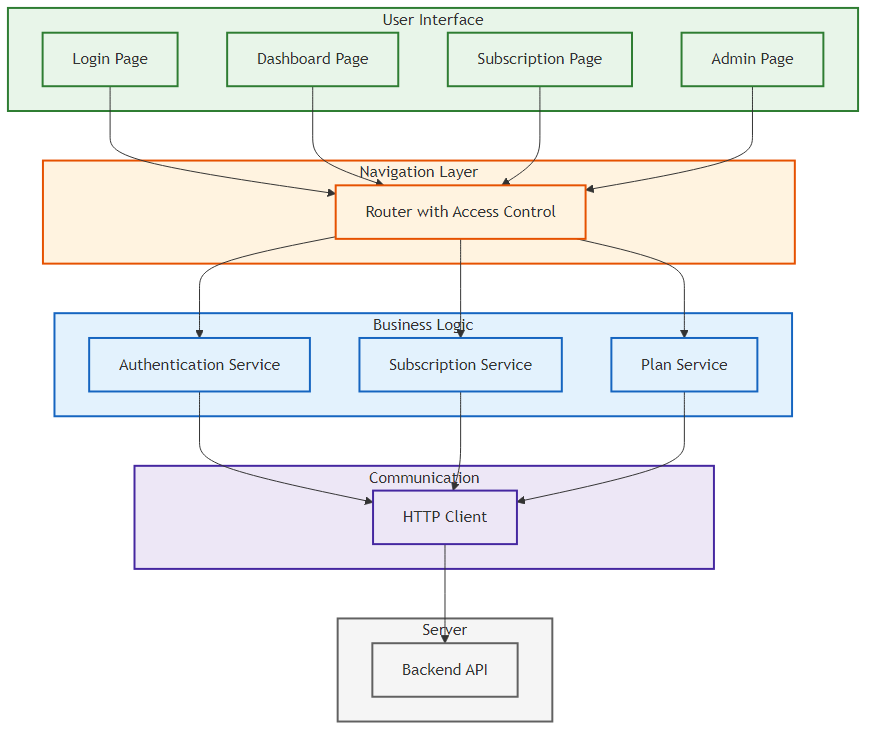
\includegraphics[width=0.8\textwidth]{images/frontend_architecture_simple.png}
\caption{Frontend Application Architecture}
\label{fig:frontend_architecture_simple}
\end{figure}

The frontend follows a clean layered architecture with clear separation of concerns. At the top, the \textbf{User Interface} layer contains the pages that users interact with (Login, Dashboard, Subscription, and Admin). The \textbf{Navigation} layer manages which pages users can access based on their authentication status and role. The \textbf{Business Logic} layer handles authentication state, subscription data, and plan information. At the bottom, the \textbf{Communication} layer sends and receives data from the backend API, automatically attaching authentication credentials to every request.

This layered approach ensures that changes in one layer (for example, updating the UI design) do not affect the underlying business logic or communication mechanisms.

\subsubsection{Technology Stack}

\begin{table}[H]
\centering
\begin{tabular}{|l|l|}
\hline
\textbf{Layer} & \textbf{Technology} \\
\hline
Frontend Framework & Vue.js 3 \\
\hline
UI Component Library & Vuetify (Material Design 3) \\
\hline
Build Tool & Vite \\
\hline
Routing & Vue Router 4 \\
\hline
\end{tabular}
\caption{Frontend Technology Stack}
\label{tab:frontend_tech_stack}
\end{table}

The application uses Vue.js 3 as the core framework for building reactive user interfaces. Vuetify provides a comprehensive set of Material Design components, ensuring a professional and consistent user experience. Vite serves as the build tool, enabling fast development and optimised production builds. Vue Router 4 manages navigation and enforces authentication constraints through navigation guards.

\input{tex/ch4_implementation/05_frontend_auth}
\input{tex/ch4_implementation/06_frontend_routing}
\subsection{Subscription Management Interface}
\label{sec:frontend_subscription}

The subscription interface provides users with tools to select service plans, complete payments through Stripe, and monitor their current usage quotas. Administrators can manage available plans through a dedicated configuration interface. The entire subscription system is built with Vue 3 components providing a responsive and interactive experience.

\subsubsection{User Subscription View}

For users with active subscriptions, the dashboard displays comprehensive subscription information:

\begin{itemize}
    \item Current plan name and subscription billing period (start and end dates)
    \item Quota allocation for both batch and real-time processing (measured in seconds or unlimited)
    \item Visual progress indicators showing current usage relative to allocated quotas
    \item Color-coded usage indicators: green for low usage, orange for moderate usage (75\%), and red for high usage (90\%+)
    \item Controls for canceling or resuming subscription at any time
    \item Scheduled plan changes with information about the next billing cycle
\end{itemize}

Usage percentages are calculated to provide clear feedback on consumption. Unlimited quotas are represented as zero usage to indicate no constraint. Plans with zero quota are displayed at 100\% to indicate the service is not available under that plan.

\subsubsection{Plan Card Component}

The plan card is a reusable interface component that displays individual subscription plan options. Each plan card shows:

\begin{itemize}
    \item Plan name and pricing retrieved from Stripe's pricing system
    \item Billing interval (monthly, annual, or one-time)
    \item Processing duration limits for both batch and live modes
    \item Feature list highlighting capabilities included in the plan
    \item Interactive button indicating action available: "Subscribe Now" for unsubscribed users, "Current Plan" for the active subscription, or "Schedule Change" to switch plans
    \item Badges indicating current or scheduled subscription status
\end{itemize}

Plan pricing is fetched dynamically from Stripe's API, ensuring the interface always displays current pricing without requiring manual updates. This integration allows changes to pricing in Stripe to be reflected immediately in the user interface.

\subsubsection{Checkout Process}

When users select a plan to purchase, the application initiates a seamless checkout process:

\begin{enumerate}
    \item User clicks the subscribe button on the desired plan card
    \item Application requests a checkout session from the backend, passing the Stripe price identifier
    \item User is redirected to Stripe's hosted checkout page
    \item User completes payment through Stripe's secure payment interface
    \item After successful payment, Stripe redirects the user back to the dashboard
    \item Application displays a success page and the subscription is activated
\end{enumerate}

If users cancel during checkout, they are returned to the dashboard on a cancellation page, allowing them to retry or select a different plan. The checkout process is entirely handled by Stripe, ensuring payment security.

\subsubsection{Subscription Management}

After purchasing a subscription, users can manage their subscription through the subscription page:

\paragraph{Plan Changes}

Users with active subscriptions can switch to different plans. The system allows scheduling plan changes at the next billing cycle rather than forcing immediate upgrades or downgrades. This prevents unexpected billing changes and allows users to plan their changes in advance.

\paragraph{Cancellation}

Users can cancel their subscriptions at any time. Cancellation is scheduled for the end of the current billing period, allowing the user to retain access for the remainder of their paid cycle. The system displays clear information about when the subscription will end.

\paragraph{Resumption}

Users who have canceled their subscription can resume it before the cancellation takes effect. This allows users to change their mind without having to re-enter payment information.

\subsubsection{Admin Plan Configuration}

Administrators access a dedicated plan management interface for configuring available subscription plans. This interface provides:

\begin{itemize}
    \item A JSON-based editor for defining plan properties including names, features, durations, and Stripe price identifiers
    \item Live validation to ensure pricing identifiers correspond to valid Stripe prices before publication
    \item Diff comparison showing what has changed from the current published version
    \item Version history tracking with ability to revert to previous configurations
    \item Real-time syntax highlighting and validation feedback
\end{itemize}

The admin editor validates each plan's Stripe price identifier against Stripe's API before allowing the configuration to be published, preventing invalid or broken pricing configurations from being saved.


\section{Summary}

This chapter described the full implementation of the Gateway Dashboard system across both backend and frontend. On the backend, the authentication system supports three login methods (email/password, Google OAuth 2.0, and Apple Sign-In) unified under a common token management layer with automatic refresh and revocation capabilities. The payment system integrates Stripe for checkout, subscription lifecycle management, plan versioning, and real time webhook synchronisation, with Redis caching to optimise plan and pricing queries. On the frontend, this project integrated new pages into the existing Gateway Dashboard, including authentication pages with SSO support, a subscription management interface with usage monitoring and plan selection, navigation guards enforcing role based access control, and an administrative interface for configuring plans and managing users. Together, these components deliver a complete, production ready platform for commercial speech service management.
